\documentclass{standalone}
\usepackage{tikz}

\begin{document}
  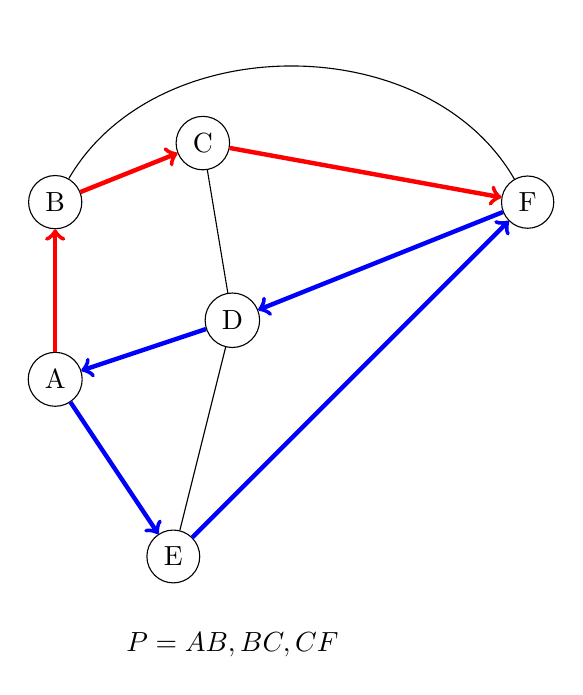
\begin{tikzpicture}[scale=0.75]
    \node[shape=circle,draw=black] (A) at (0,0) {A};
    \node[shape=circle,draw=black] (B) at (0,3) {B};
    \node[shape=circle,draw=black] (C) at (2.5,4) {C};
    \node[shape=circle,draw=black] (D) at (3,1) {D};
    \node[shape=circle,draw=black] (E) at (2,-3) {E};
    \node[shape=circle,draw=black] (F) at (8,3) {F} ;
    \node (P) at (3,-4.5) {\(P=AB,BC,CF\)};

    \path [->] (A) edge [ultra thick,red] (B);
    \path [->] (B) edge [ultra thick,red] (C);
    \path (B) edge [bend left=60] (F);
    \path [<-] (A) edge [ultra thick,blue] (D);
    \path (D) edge (C);
    \path [->] (A) edge [ultra thick,blue] (E);
    \path (D) edge (E);
    \path [<-] (D) edge [ultra thick,blue] (F);
    \path [->] (C) edge [ultra thick,red] (F);
    \path [->] (E) edge [ultra thick,blue] (F);
  \end{tikzpicture}
\end{document}
